\documentclass{beamer}
\hypersetup{bookmarksdepth=5}

\usepackage[T1]{fontenc}   % required for luximono!
\usepackage{lmodern}
\usepackage[scaled=0.8]{luximono}  % typewriter font with bold face

% To install the luximono font files:
% getnonfreefonts-sys --all        or
% getnonfreefonts-sys luximono
%
% when there are trouble you might need to:
% - Create /etc/texmf/updmap.d/99local-luximono.cfg
%   containing the single line: Map ul9.map
% - Run update-updmap followed by mktexlsr and updmap-sys
%
% This commands must be executed as root with a root environment
% (i.e. run "sudo su" and then execute the commands in the root
% shell, don't just prefix the commands with "sudo").

% formats the text according the set language
\usepackage[english]{babel}
\usepackage{amsmath}
\usepackage{multirow}
\usepackage{booktabs}
\usepackage{listings}
\usepackage{setspace}
\usepackage{skull}
\usepackage{units}

\usepackage{tikz}
\usetikzlibrary{calc}
\usetikzlibrary{arrows}
\usetikzlibrary{scopes}
\usetikzlibrary{through}
\usetikzlibrary{shapes.geometric}

\lstset{basicstyle=\ttfamily}

\def\B#1{{\tt\textbackslash{}#1}}
\def\C#1{\lstinline[language=C++]{#1}}
\def\V#1{\lstinline[language=Verilog]{#1}}

\lstdefinelanguage{liberty}{
	morecomment=[s]{/*}{*/},
	morekeywords={library,cell,area,pin,direction,function,clocked_on,next_state,clock,ff},
	morestring=[b]",
}

\lstdefinelanguage{rtlil}{
	morecomment=[l]{\#},
	morekeywords={module,attribute,parameter,wire,memory,auto,width,offset,size,input,output,inout,cell,connect,switch,case,assign,sync,low,high,posedge,negedge,edge,always,update,process,end},
	morestring=[b]",
}

\lstdefinelanguage{ys}{
	morecomment=[l]{\#},
}

\lstset{
	commentstyle=\color{YosysGreen},
}

\newenvironment{boxalertenv}{\begin{altenv}%
{\usebeamertemplate{alerted text begin}\usebeamercolor[fg]{alerted text}\usebeamerfont{alerted text}\setlength{\fboxsep}{1pt}\colorbox{bg}}
{\usebeamertemplate{alerted text end}}{\color{.}}{}}{\end{altenv}}

\newcommand<>{\boxalert}[1]{{%
\begin{boxalertenv}#2{#1}\end{boxalertenv}%
}}

\newcommand{\subsectionpagesuffix}{
\vfill\begin{centering}
{\usebeamerfont{subsection name}\usebeamercolor[fg]{subsection name}of \sectionname~\insertsectionnumber}
\vskip1em\par
\setbeamercolor{graybox}{bg=gray}
\begin{beamercolorbox}[sep=8pt,center]{graybox}
\usebeamerfont{subsection title}\insertsection\par
\end{beamercolorbox}
\end{centering}}

\title{Yosys Open SYnthesis Suite}
\author{Clifford Wolf}
\institute{http://www.clifford.at/yosys/}

\usetheme{Madrid}
\usecolortheme{seagull}
\beamertemplatenavigationsymbolsempty

\definecolor{YosysGreen}{RGB}{85,136,102}
\definecolor{MyBlue}{RGB}{85,130,180}

\setbeamercolor{title}{fg=black,bg=YosysGreen!70}
\setbeamercolor{titlelike}{fg=black,bg=YosysGreen!70}
\setbeamercolor{frametitle}{fg=black,bg=YosysGreen!70}
\setbeamercolor{block title}{fg=black,bg=YosysGreen!70}
\setbeamercolor{item projected}{fg=black,bg=YosysGreen}

\begin{document}

\begin{frame}
\titlepage
\end{frame}

\setcounter{section}{-3}

\section{Abstract}
\begin{frame}{Abstract}
Yosys is the first full-featured open source software for Verilog HDL
synthesis. It supports most of Verilog-2005 and is well tested with
real-world designs from the ASIC and FPGA world.

\bigskip
Learn how to use Yosys to create your own custom synthesis flows and
discover why open source HDL synthesis is important for researchers,
hobbyists, educators and engineers alike.

\bigskip
This presentation covers basic concepts of Yosys, writing synthesis scripts
for a wide range of applications, creating Yosys scripts for various
non-synthesis applications (such as formal equivalence checking) and
writing extensions to Yosys using the C++ API.
\end{frame}

\section{About me}
\begin{frame}{About me}
Hi! I'm Clifford Wolf.

\bigskip
I like writing open source software. For example:
\begin{itemize}
\item Yosys
\item OpenSCAD (now maintained by Marius Kintel)
\item SPL (a not very popular scripting language)
\item EmbedVM (a very simple compiler+vm for 8 bit micros)
\item Lib(X)SVF (a library to play SVF/XSVF files over JTAG)
\item ROCK Linux (discontinued since 2010)
\end{itemize}
\end{frame}

\section{Outline}
\begin{frame}{Outline}
Yosys is an Open Source Verilog synthesis tool, and more.

\bigskip
Outline of this presentation:
\begin{itemize}
\item Introduction to the field and Yosys
\item Yosys by example: synthesis
\item Yosys by example: advanced synthesis
\item Yosys by example: beyond synthesis
\item Writing Yosys extensions in C++
\end{itemize}
\end{frame}


\section{Introduction to Yosys}

\begin{frame}
\sectionpage
\end{frame}

\iffalse
%%%%%%%%%%%%%%%%%%%%%%%%%%%%%%%%%%%%%%%%%%%%%%%%%%%%%%%%%%%%%%%%%%%%%%%%%%%%%

\subsection{Example Project}

\begin{frame}[t]{\subsecname}
The following slides cover an example project. This project contains three files:
\begin{itemize}
\item A simple ASIC synthesis script
\item A digital design written in Verilog
\item A simple CMOS cell library
\end{itemize}
\vfill
Direct link to the files: \\ \footnotesize
\url{https://github.com/YosysHQ/yosys/tree/master/manual/PRESENTATION_Intro}
\end{frame}

%%%%%%%%%%%%%%%%%%%%%%%%%%%%%%%%%%%%%%%%%%%%%%%%%%%%%%%%%%%%%%%%%%%%%%%%%%%%%

\subsection{The synth command}

\begin{frame}[fragile]{\subsecname{}}
Yosys contains a default (recommended example) synthesis script in form of the
{\tt synth} command. The following commands are executed by this synthesis command:

\begin{columns}
\column[t]{5cm}
\begin{lstlisting}[xleftmargin=1cm, basicstyle=\ttfamily\fontsize{8pt}{10pt}\selectfont, language=ys]
begin:
    hierarchy -check [-top <top>]

coarse:
    proc
    opt
    wreduce
    alumacc
    share
    opt
    fsm
    opt -fast
    memory -nomap
    opt_clean
\end{lstlisting}
\column[t]{5cm}
\begin{lstlisting}[xleftmargin=1cm, basicstyle=\ttfamily\fontsize{8pt}{10pt}\selectfont, language=ys]
fine:
    opt -fast -full
    memory_map
    opt -full
    techmap
    opt -fast

abc:
    abc -fast
    opt -fast
\end{lstlisting}
\end{columns}
\end{frame}

%%%%%%%%%%%%%%%%%%%%%%%%%%%%%%%%%%%%%%%%%%%%%%%%%%%%%%%%%%%%%%%%%%%%%%%%%%%%%

\subsection{Yosys Commands}

\begin{frame}[fragile]{\subsecname{} 1/3 \hspace{0pt plus 1 filll} (excerpt)}
Command reference:
\begin{itemize}
\item Use ``{\tt help}'' for a command list and ``{\tt help \it command}'' for details.
\item Or run ``{\tt yosys -H}'' or ``{\tt yosys -h \it command}''.
\item Or go to \url{https://yosyshq.net/yosys/documentation.html}.
\end{itemize}

\bigskip
Commands for design navigation and investigation:
\begin{lstlisting}[xleftmargin=1cm, basicstyle=\ttfamily\fontsize{8pt}{10pt}\selectfont, language=ys]
    cd                   # a shortcut for 'select -module <name>'
    ls                   # list modules or objects in modules
    dump                 # print parts of the design in RTLIL format
    show                 # generate schematics using graphviz
    select               # modify and view the list of selected objects
\end{lstlisting}

\bigskip
Commands for executing scripts or entering interactive mode:
\begin{lstlisting}[xleftmargin=1cm, basicstyle=\ttfamily\fontsize{8pt}{10pt}\selectfont, language=ys]
    shell                # enter interactive command mode
    history              # show last interactive commands
    script               # execute commands from script file
    tcl                  # execute a TCL script file
\end{lstlisting}
\end{frame}

\begin{frame}[fragile]{\subsecname{} 2/3 \hspace{0pt plus 1 filll} (excerpt)}
Commands for reading and elaborating the design:
\begin{lstlisting}[xleftmargin=1cm, basicstyle=\ttfamily\fontsize{8pt}{10pt}\selectfont, language=ys]
    read_rtlil           # read modules from RTLIL file
    read_verilog         # read modules from Verilog file
    hierarchy            # check, expand and clean up design hierarchy
\end{lstlisting}

\bigskip
Commands for high-level synthesis:
\begin{lstlisting}[xleftmargin=1cm, basicstyle=\ttfamily\fontsize{8pt}{10pt}\selectfont, language=ys]
    proc                 # translate processes to netlists
    fsm                  # extract and optimize finite state machines
    memory               # translate memories to basic cells
    opt                  # perform simple optimizations
\end{lstlisting}

\bigskip
Commands for technology mapping:
\begin{lstlisting}[xleftmargin=1cm, basicstyle=\ttfamily\fontsize{8pt}{10pt}\selectfont, language=ys]
    techmap              # generic technology mapper
    abc                  # use ABC for technology mapping
    dfflibmap            # technology mapping of flip-flops
    hilomap              # technology mapping of constant hi- and/or lo-drivers
    iopadmap             # technology mapping of i/o pads (or buffers)
    flatten              # flatten design
\end{lstlisting}
\end{frame}

\begin{frame}[fragile]{\subsecname{} 3/3 \hspace{0pt plus 1 filll} (excerpt)}
Commands for writing the results:
\begin{lstlisting}[xleftmargin=1cm, basicstyle=\ttfamily\fontsize{8pt}{10pt}\selectfont, language=ys]
    write_blif           # write design to BLIF file
    write_btor           # write design to BTOR file
    write_edif           # write design to EDIF netlist file
    write_rtlil          # write design to RTLIL file
    write_spice          # write design to SPICE netlist file
    write_verilog        # write design to Verilog file
\end{lstlisting}

\bigskip
Script-Commands for standard synthesis tasks:
\begin{lstlisting}[xleftmargin=1cm, basicstyle=\ttfamily\fontsize{8pt}{10pt}\selectfont, language=ys]
    synth                # generic synthesis script
    synth_xilinx         # synthesis for Xilinx FPGAs
\end{lstlisting}

\bigskip
Commands for model checking:
\begin{lstlisting}[xleftmargin=1cm, basicstyle=\ttfamily\fontsize{8pt}{10pt}\selectfont, language=ys]
    sat                  # solve a SAT problem in the circuit
    miter                # automatically create a miter circuit
    scc                  # detect strongly connected components (logic loops)
\end{lstlisting}

\bigskip
... and many many more.
\end{frame}

%%%%%%%%%%%%%%%%%%%%%%%%%%%%%%%%%%%%%%%%%%%%%%%%%%%%%%%%%%%%%%%%%%%%%%%%%%%%%

\subsection{More Verilog Examples}

\begin{frame}[fragile]{\subsecname{} 1/3}
\begin{lstlisting}[xleftmargin=1cm, basicstyle=\ttfamily\fontsize{8pt}{10pt}\selectfont, language=Verilog]
module detectprime(a, y);
    input [4:0] a;
    output y;

    integer i, j;
    reg [31:0] lut;

    initial begin
        for (i = 0; i < 32; i = i+1) begin
            lut[i] = i > 1;
            for (j = 2; j*j <= i; j = j+1)
                if (i % j == 0)
                    lut[i] = 0;
        end
    end

    assign y = lut[a];
endmodule
\end{lstlisting}
\end{frame}

\begin{frame}[fragile]{\subsecname{} 2/3}
\begin{lstlisting}[xleftmargin=1cm, basicstyle=\ttfamily\fontsize{8pt}{10pt}\selectfont, language=Verilog]
module carryadd(a, b, y);
    parameter WIDTH = 8;
    input [WIDTH-1:0] a, b;
    output [WIDTH-1:0] y;

    genvar i;
    generate
        for (i = 0; i < WIDTH; i = i+1) begin:STAGE
            wire IN1 = a[i], IN2 = b[i];
            wire C, Y;
            if (i == 0)
                assign C = IN1 & IN2, Y = IN1 ^ IN2;
            else
                assign C = (IN1 & IN2) | ((IN1 | IN2) & STAGE[i-1].C),
                       Y = IN1 ^ IN2 ^ STAGE[i-1].C;
            assign y[i] = Y;
        end
    endgenerate
endmodule
\end{lstlisting}
\end{frame}

\begin{frame}[fragile]{\subsecname{} 3/3}
\begin{lstlisting}[xleftmargin=1cm, basicstyle=\ttfamily\fontsize{7pt}{8.5pt}\selectfont, language=Verilog]
module cam(clk, wr_enable, wr_addr, wr_data, rd_data, rd_addr, rd_match);
    parameter WIDTH = 8;
    parameter DEPTH = 16;
    localparam ADDR_BITS = $clog2(DEPTH-1);

    input clk, wr_enable;
    input [ADDR_BITS-1:0] wr_addr;
    input [WIDTH-1:0] wr_data, rd_data;
    output reg [ADDR_BITS-1:0] rd_addr;
    output reg rd_match;

    integer i;
    reg [WIDTH-1:0] mem [0:DEPTH-1];

    always @(posedge clk) begin
        rd_addr <= 'bx;
        rd_match <= 0;
        for (i = 0; i < DEPTH; i = i+1)
            if (mem[i] == rd_data) begin
                rd_addr <= i;
                rd_match <= 1;
            end
        if (wr_enable)
            mem[wr_addr] <= wr_data;
    end
endmodule
\end{lstlisting}
\end{frame}

%%%%%%%%%%%%%%%%%%%%%%%%%%%%%%%%%%%%%%%%%%%%%%%%%%%%%%%%%%%%%%%%%%%%%%%%%%%%%

\subsection{Currently unsupported Verilog-2005 language features}

\begin{frame}{\subsecname}
\begin{itemize}
\item Tri-state logic
\item The wor/wand wire types (maybe for 0.5)
\item Latched logic (is synthesized as logic with feedback loops)
\item Some non-synthesizable features that should be ignored in synthesis are not supported by the parser and cause a parser error (file a bug report if you encounter this problem)
\end{itemize}
\end{frame}

%%%%%%%%%%%%%%%%%%%%%%%%%%%%%%%%%%%%%%%%%%%%%%%%%%%%%%%%%%%%%%%%%%%%%%%%%%%%%

\subsection{Verification of Yosys}

\begin{frame}{\subsecname}
Continuously checking the correctness of Yosys and making sure that new features
do not break old ones is a high priority in Yosys.

\bigskip
Two external test suites have been built for Yosys: VlogHammer and yosys-bigsim
(see next slides)

\bigskip
In addition to that, yosys comes with $\approx\!200$ test cases used in ``{\tt make test}''.

\bigskip
A debug build of Yosys also contains a lot of asserts and checks the integrity of
the internal state after each command.
\end{frame}

\begin{frame}[fragile]{\subsecname{} -- VlogHammer}
VlogHammer is a Verilog regression test suite developed to test the different
subsystems in Yosys by comparing them to each other and to the output created
by some other tools (Xilinx Vivado, Xilinx XST, Altera Quartus II, ...).

\bigskip
Yosys Subsystems tested: Verilog frontend, const folding, const eval, technology mapping,
simulation models, SAT models.

\bigskip
Thousands of auto-generated test cases containing code such as:
\begin{lstlisting}[xleftmargin=1cm, basicstyle=\ttfamily\fontsize{8pt}{10pt}\selectfont, language=Verilog]
assign y9 = $signed(((+$signed((^(6'd2 ** a2))))<$unsigned($unsigned(((+a3))))));
assign y10 = (-((+((+{2{(~^p13)}})))^~(!{{b5,b1,a0},(a1&p12),(a4+a3)})));
assign y11 = (~&(-{(-3'sd3),($unsigned($signed($unsigned({p0,b4,b1}))))}));
\end{lstlisting}

\bigskip
Some bugs in Yosys where found and fixed thanks to VlogHammer. Over 50 bugs in
the other tools used as external reference where found and reported so far.
\end{frame}

\begin{frame}{\subsecname{} -- yosys-bigsim}
yosys-bigsim is a collection of real-world open-source Verilog designs and test
benches. yosys-bigsim compares the testbench outputs of simulations of the original
Verilog code and synthesis results.

\bigskip
The following designs are included in yosys-bigsim (excerpt):
\begin{itemize}
\item {\tt openmsp430} -- an MSP430 compatible 16 bit CPU
\item {\tt aes\_5cycle\_2stage} -- an AES encryption core
\item {\tt softusb\_navre} -- an AVR compatible 8 bit CPU
\item {\tt amber23} -- an ARMv2 compatible 32 bit CPU
\item {\tt lm32} -- another 32 bit CPU from Lattice Semiconductor
\item {\tt verilog-pong} -- a hardware pong game with VGA output
\item {\tt elliptic\_curve\_group} -- ECG point-add and point-scalar-mul core
\item {\tt reed\_solomon\_decoder} -- a Reed-Solomon Error Correction Decoder
\end{itemize}
\end{frame}

%%%%%%%%%%%%%%%%%%%%%%%%%%%%%%%%%%%%%%%%%%%%%%%%%%%%%%%%%%%%%%%%%%%%%%%%%%%%%

\subsection{Benefits of Open Source HDL Synthesis}

\begin{frame}{\subsecname}
\begin{itemize}
\item Cost (also applies to ``free as in free beer'' solutions)
\item Availability and Reproducibility
\item Framework- and all-in-one-aspects
\item Educational Tool
\end{itemize}

\bigskip

Yosys is open source under the ISC license.
\end{frame}

\begin{frame}{\subsecname{} -- 1/3}
\begin{itemize}
\item Cost (also applies to ``free as in free beer'' solutions): \smallskip\par
Today the cost for a mask set in $\unit[180]{nm}$ technology is far less than
the cost for the design tools needed to design the mask layouts. Open Source
ASIC flows are an important enabler for ASIC-level Open Source Hardware.

\bigskip
\item Availability and Reproducibility: \smallskip\par
If you are a researcher who is publishing, you want to use tools that everyone
else can also use. Even if most universities have access to all major
commercial tools, you usually do not have easy access to the version that was
used in a research project a couple of years ago. With Open Source tools you
can even release the source code of the tool you have used alongside your data.
\end{itemize}
\end{frame}

\begin{frame}{\subsecname{} -- 2/3}
\begin{itemize}
\item Framework: \smallskip\par
Yosys is not only a tool. It is a framework that can be used as basis for other
developments, so researchers and hackers alike do not need to re-invent the
basic functionality. Extensibility was one of Yosys' design goals.

\bigskip
\item All-in-one: \smallskip\par
Because of the framework characteristics of Yosys, an increasing number of features
become available in one tool. Yosys not only can be used for circuit synthesis but
also for formal equivalence checking, SAT solving, and for circuit analysis, to
name just a few other application domains. With proprietary software one needs to
learn a new tool for each of these applications.
\end{itemize}
\end{frame}

\begin{frame}{\subsecname{} -- 3/3}
\begin{itemize}
\item Educational Tool: \smallskip\par
Proprietary synthesis tools are at times very secretive about their inner
workings. They often are ``black boxes''. Yosys is very open about its
internals and it is easy to observe the different steps of synthesis.
\end{itemize}

\bigskip
\begin{block}{Yosys is licensed under the ISC license:}
Permission to use, copy, modify, and/or distribute this software for any
purpose with or without fee is hereby granted, provided that the above
copyright notice and this permission notice appear in all copies.
\end{block}
\end{frame}

%%%%%%%%%%%%%%%%%%%%%%%%%%%%%%%%%%%%%%%%%%%%%%%%%%%%%%%%%%%%%%%%%%%%%%%%%%%%%

\subsection{Typical Applications for Yosys}

\begin{frame}{\subsecname}
\begin{itemize}
\item Synthesis of final production designs
\item Pre-production synthesis (trial runs before investing in other tools)
\item Conversion of full-featured Verilog to simple Verilog
\item Conversion of Verilog to other formats (BLIF, BTOR, etc)
\item Demonstrating synthesis algorithms (e.g. for educational purposes)
\item Framework for experimenting with new algorithms
\item Framework for building custom flows\footnote[frame]{Not limited to synthesis
but also formal verification, reverse engineering, ...}
\end{itemize}
\end{frame}

%%%%%%%%%%%%%%%%%%%%%%%%%%%%%%%%%%%%%%%%%%%%%%%%%%%%%%%%%%%%%%%%%%%%%%%%%%%%%

\subsection{Projects (that I know of) using Yosys}

\begin{frame}{\subsecname{} -- (1/2)}
\begin{itemize}
\item Ongoing PhD project on coarse grain synthesis \\
{\setlength{\parindent}{0.5cm}\footnotesize
Johann Glaser and C. Wolf. Methodology and Example-Driven Interconnect
Synthesis for Designing Heterogeneous Coarse-Grain Reconfigurable
Architectures. In Jan Haase, editor, \it Models, Methods, and Tools for Complex
Chip Design. Lecture Notes in Electrical Engineering. Volume 265, 2014, pp
201-221. Springer, 2013.}

\bigskip
\item I know several people that use Yosys simply as Verilog frontend for other
flows (using either the BLIF and BTOR backends).

\bigskip
\item I know some analog chip designers that use Yosys for small digital
control logic because it is simpler than setting up a commercial flow.
\end{itemize}
\end{frame}

\begin{frame}{\subsecname{} -- (2/2)}
\begin{itemize}
\item Efabless
\begin{itemize}
\smallskip \item Not much information on the website (\url{http://efabless.com}) yet.
\smallskip \item Very cheap 180nm prototyping process (partnering with various fabs)
\smallskip \item A semiconductor company, NOT an EDA company
\smallskip \item Web-based design environment
\smallskip \item HDL Synthesis using Yosys
\smallskip \item Custom place\&route tool

\bigskip
\item efabless is building an Open Source IC as reference design. \\
\hskip1cm (to be announced soon: \url{http://www.openic.io})
\end{itemize}
\end{itemize}
\end{frame}

%%%%%%%%%%%%%%%%%%%%%%%%%%%%%%%%%%%%%%%%%%%%%%%%%%%%%%%%%%%%%%%%%%%%%%%%%%%%%

\subsection{Supported Platforms}

\begin{frame}{\subsecname}
\begin{itemize}
\item Main development OS: Kubuntu 14.04
\item There is a PPA for ubuntu (not maintained by me)
\item Any current Debian-based system should work out of the box
\item When building on other Linux distributions:
\begin{itemize}
\item Needs compiler with some C++11 support
\item See README file for build instructions
\item Post to the subreddit if you get stuck
\end{itemize}
\item Ported to OS X (Darwin) and OpenBSD
\item Native win32 build with VisualStudio
\item Cross win32 build with MXE
\end{itemize}
\end{frame}

%%%%%%%%%%%%%%%%%%%%%%%%%%%%%%%%%%%%%%%%%%%%%%%%%%%%%%%%%%%%%%%%%%%%%%%%%%%%%

\subsection{Other Open Source Tools}

\begin{frame}{\subsecname}
\begin{itemize}
\item Icarus Verilog \\
\smallskip\hskip1cm{}Verilog Simulation (and also a good syntax checker) \\
\smallskip\hskip1cm{}\url{http://iverilog.icarus.com/}

\bigskip
\item Qflow (incl. TimberWolf, qrouter and Magic) \\
\smallskip\hskip1cm{}A complete ASIC synthesis flow, using Yosys and ABC \\
\smallskip\hskip1cm{}\url{http://opencircuitdesign.com/qflow/}

\bigskip
\item ABC \\
\smallskip\hskip1cm{}Logic optimization, technology mapping, and more \\
\smallskip\hskip1cm{}\url{http://www.eecs.berkeley.edu/~alanmi/abc/}
\end{itemize}
\end{frame}

%%%%%%%%%%%%%%%%%%%%%%%%%%%%%%%%%%%%%%%%%%%%%%%%%%%%%%%%%%%%%%%%%%%%%%%%%%%%%

\subsection{Yosys needs you}

\begin{frame}{\subsecname}
\dots as an active user:
\begin{itemize}
\item Use Yosys for on your own projects
\item .. even if you are not using it as final synthesis tool
\item Join the discussion on the Subreddit
\item Report bugs and send in feature requests
\end{itemize}

\bigskip
\dots as a developer:
\begin{itemize}
\item Use Yosys as environment for your (research) work
\item .. you might also want to look into ABC for logic-level stuff
\item Fork the project on github or create loadable plugins
\item We need a VHDL frontend or a good VHDL-to-Verilog converter
\end{itemize}
\end{frame}

%%%%%%%%%%%%%%%%%%%%%%%%%%%%%%%%%%%%%%%%%%%%%%%%%%%%%%%%%%%%%%%%%%%%%%%%%%%%%

\subsection{Documentation, Downloads, Contacts}

\begin{frame}{\subsecname}
\begin{itemize}
\item Website: \\
\smallskip\hskip1cm\url{https://yosyshq.net/yosys/}

\bigskip
\item Manual, Command Reference, Application Notes: \\
\smallskip\hskip1cm\url{https://yosyshq.net/yosys/documentation.html}

\bigskip
\item Instead of a mailing list we have a SubReddit: \\
\smallskip\hskip1cm\url{http://www.reddit.com/r/yosys/}

\bigskip
\item Direct link to the source code: \\
\smallskip\hskip1cm\url{https://github.com/YosysHQ/yosys}
\end{itemize}
\end{frame}

%%%%%%%%%%%%%%%%%%%%%%%%%%%%%%%%%%%%%%%%%%%%%%%%%%%%%%%%%%%%%%%%%%%%%%%%%%%%%

\subsection{Summary}

\begin{frame}{\subsecname}
\begin{itemize}
\item Yosys is a powerful tool and framework for Verilog synthesis.
\item It uses a command-based interface and can be controlled by scripts.
\item By combining existing commands and implementing new commands Yosys can
be used in a wide range of application far beyond simple synthesis.
\end{itemize}

\bigskip
\bigskip
\begin{center}
Questions?
\end{center}

\bigskip
\bigskip
\begin{center}
\url{https://yosyshq.net/yosys/}
\end{center}
\end{frame}



\section{Yosys by example -- Synthesis}

\begin{frame}
\sectionpage
\end{frame}

%%%%%%%%%%%%%%%%%%%%%%%%%%%%%%%%%%%%%%%%%%%%%%%%%%%%%%%%%%%%%%%%%%%%%%%%%%%%%

\subsection{Typical Phases of a Synthesis Flow}

\begin{frame}{\subsecname}
TBD
\end{frame}

%%%%%%%%%%%%%%%%%%%%%%%%%%%%%%%%%%%%%%%%%%%%%%%%%%%%%%%%%%%%%%%%%%%%%%%%%%%%%

\subsection{Design elaboration}

\begin{frame}{\subsecname}
TBD
\end{frame}

%%%%%%%%%%%%%%%%%%%%%%%%%%%%%%%%%%%%%%%%%%%%%%%%%%%%%%%%%%%%%%%%%%%%%%%%%%%%%

\subsection{High-Level Synthesis}

\begin{frame}{\subsecname}
TBD
\end{frame}

%%%%%%%%%%%%%%%%%%%%%%%%%%%%%%%%%%%%%%%%%%%%%%%%%%%%%%%%%%%%%%%%%%%%%%%%%%%%%

\subsection{The ``proc'' commands}

\begin{frame}{\subsecname}
TBD
\end{frame}

%%%%%%%%%%%%%%%%%%%%%%%%%%%%%%%%%%%%%%%%%%%%%%%%%%%%%%%%%%%%%%%%%%%%%%%%%%%%%

\subsection{The ``memory'' commands}

\begin{frame}{\subsecname}
TBD
\end{frame}

%%%%%%%%%%%%%%%%%%%%%%%%%%%%%%%%%%%%%%%%%%%%%%%%%%%%%%%%%%%%%%%%%%%%%%%%%%%%%

\subsection{The ``fsm'' commands}

\begin{frame}{\subsecname}
TBD
\end{frame}

%%%%%%%%%%%%%%%%%%%%%%%%%%%%%%%%%%%%%%%%%%%%%%%%%%%%%%%%%%%%%%%%%%%%%%%%%%%%%

\subsection{Low-Level Synthesis}

\begin{frame}{\subsecname}
TBD
\end{frame}

%%%%%%%%%%%%%%%%%%%%%%%%%%%%%%%%%%%%%%%%%%%%%%%%%%%%%%%%%%%%%%%%%%%%%%%%%%%%%

\subsection{The ``techmap'' command}

\begin{frame}{\subsecname}
TBD
\end{frame}

%%%%%%%%%%%%%%%%%%%%%%%%%%%%%%%%%%%%%%%%%%%%%%%%%%%%%%%%%%%%%%%%%%%%%%%%%%%%%

\subsection{The ``abc'' command}

\begin{frame}{\subsecname}
TBD
\end{frame}

%%%%%%%%%%%%%%%%%%%%%%%%%%%%%%%%%%%%%%%%%%%%%%%%%%%%%%%%%%%%%%%%%%%%%%%%%%%%%

\subsection{Other special-purpose mapping commands}

\begin{frame}{\subsecname}
TBD
\end{frame}

%%%%%%%%%%%%%%%%%%%%%%%%%%%%%%%%%%%%%%%%%%%%%%%%%%%%%%%%%%%%%%%%%%%%%%%%%%%%%



\section{Yosys by example -- Advanced Synthesis}

\begin{frame}
\sectionpage
\end{frame}

%%%%%%%%%%%%%%%%%%%%%%%%%%%%%%%%%%%%%%%%%%%%%%%%%%%%%%%%%%%%%%%%%%%%%%%%%%%%%



\section{Yosys by example -- Beyond Synthesis}

\begin{frame}
\sectionpage
\end{frame}

\begin{frame}{Overview}
This section contains 3 subsections:
\begin{itemize}
\item Interactive Design Investigation
\item Symbolic Model Checking
\item Reverse Engineering
\end{itemize}
\end{frame}

%%%%%%%%%%%%%%%%%%%%%%%%%%%%%%%%%%%%%%%%%%%%%%%%%%%%%%%%%%%%%%%%%%%%%%%%%%%%%

\subsection{Interactive Design Investigation}

\begin{frame}
\subsectionpage
\subsectionpagesuffix
\end{frame}

\subsubsection{TBD}

\begin{frame}{\subsubsecname}
TBD
\end{frame}

%%%%%%%%%%%%%%%%%%%%%%%%%%%%%%%%%%%%%%%%%%%%%%%%%%%%%%%%%%%%%%%%%%%%%%%%%%%%%

\subsection{Symbolic Model Checking}

\begin{frame}
\subsectionpage
\subsectionpagesuffix
\end{frame}

\subsubsection{TBD}

\begin{frame}{\subsubsecname}
TBD
\end{frame}

%%%%%%%%%%%%%%%%%%%%%%%%%%%%%%%%%%%%%%%%%%%%%%%%%%%%%%%%%%%%%%%%%%%%%%%%%%%%%

\subsection{Reverse Engineering}

\begin{frame}
\subsectionpage
\subsectionpagesuffix
\end{frame}

\subsubsection{TBD}

\begin{frame}{\subsubsecname}
TBD
\end{frame}

%%%%%%%%%%%%%%%%%%%%%%%%%%%%%%%%%%%%%%%%%%%%%%%%%%%%%%%%%%%%%%%%%%%%%%%%%%%%%

\subsection{Summary}

\begin{frame}{\subsecname}
\begin{itemize}
\item TBD
\item TBD
\item TBD
\item TBD
\end{itemize}

\bigskip
\bigskip
\begin{center}
Questions?
\end{center}

\bigskip
\bigskip
\begin{center}
\url{http://www.clifford.at/yosys/}
\end{center}
\end{frame}



\section{Programming Yosys Extensions}

\begin{frame}
\sectionpage
\end{frame}

%%%%%%%%%%%%%%%%%%%%%%%%%%%%%%%%%%%%%%%%%%%%%%%%%%%%%%%%%%%%%%%%%%%%%%%%%%%%%

\subsection{Program Components and Data Formats}

\begin{frame}{\subsecname}
\begin{center}
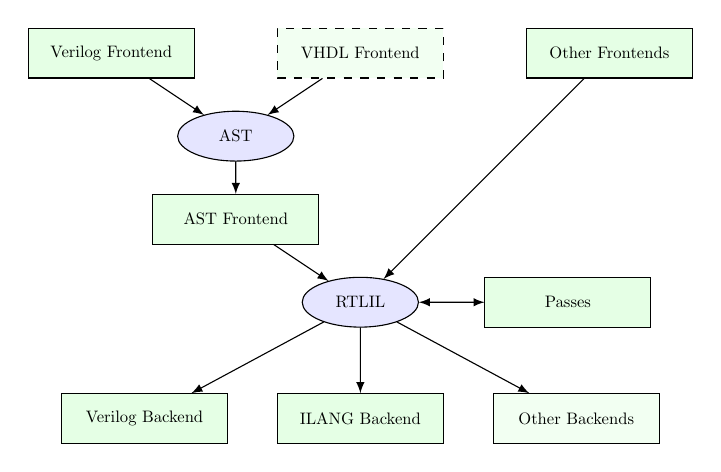
\begin{tikzpicture}[scale=0.6, every node/.style={transform shape}]
	\tikzstyle{process} = [draw, fill=green!10, rectangle, minimum height=3em, minimum width=10em, node distance=15em]
	\tikzstyle{data} = [draw, fill=blue!10, ellipse, minimum height=3em, minimum width=7em, node distance=15em]
	\node[process] (vlog) {Verilog Frontend};
	\node[process, dashed, fill=green!5] (vhdl) [right of=vlog] {VHDL Frontend};
	\node[process] (ilang) [right of=vhdl] {Other Frontends};
	\node[data] (ast) [below of=vlog, node distance=5em, xshift=7.5em] {AST};
	\node[process] (astfe) [below of=ast, node distance=5em] {AST Frontend};
	\node[data] (rtlil) [below of=astfe, node distance=5em, xshift=7.5em] {RTLIL};
	\node[process] (pass) [right of=rtlil, node distance=5em, xshift=7.5em] {Passes};
	\node[process] (vlbe) [below of=rtlil, node distance=7em, xshift=-13em] {Verilog Backend};
	\node[process] (ilangbe) [below of=rtlil, node distance=7em, xshift=0em] {ILANG Backend};
	\node[process, fill=green!5] (otherbe) [below of=rtlil, node distance=7em, xshift=+13em] {Other Backends};

	\draw[-latex] (vlog) -- (ast);
	\draw[-latex] (vhdl) -- (ast);
	\draw[-latex] (ast) -- (astfe);
	\draw[-latex] (astfe) -- (rtlil);
	\draw[-latex] (ilang) -- (rtlil);
	\draw[latex-latex] (rtlil) -- (pass);
	\draw[-latex] (rtlil) -- (vlbe);
	\draw[-latex] (rtlil) -- (ilangbe);
	\draw[-latex] (rtlil) -- (otherbe);
\end{tikzpicture}
\end{center}
\end{frame}

%%%%%%%%%%%%%%%%%%%%%%%%%%%%%%%%%%%%%%%%%%%%%%%%%%%%%%%%%%%%%%%%%%%%%%%%%%%%%

\subsection{Simplified RTLIL Entity-Relationship Diagram}

\begin{frame}{\subsecname}
Between passses and frontends/backends the design in stored in Yosys' internal RTLIL (RTL Intermediate Language) format. For
writing Yosys extensions it is key to understand this format.

\bigskip
\begin{center}
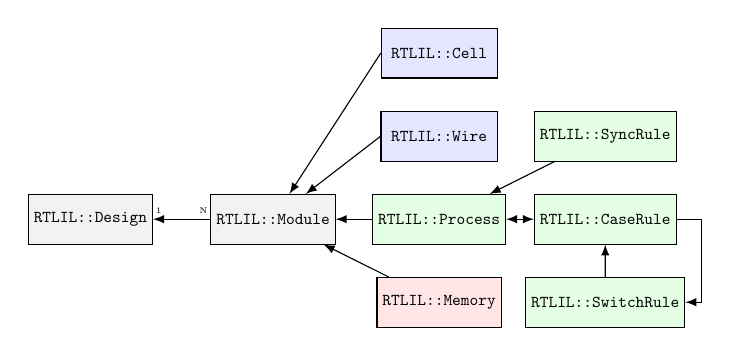
\begin{tikzpicture}[scale=0.6, every node/.style={transform shape}]
	\tikzstyle{entity} = [draw, fill=gray!10, rectangle, minimum height=3em, minimum width=7em, node distance=5em, font={\ttfamily}]
	\node[entity] (design) {RTLIL::Design};
	\node[entity] (module) [right of=design, node distance=11em] {RTLIL::Module} edge [-latex] node[above] {\tiny 1 \hskip3em N} (design);

	\node[entity] (process) [fill=green!10, right of=module, node distance=10em] {RTLIL::Process} (process.west) edge [-latex] (module);
	\node[entity] (memory) [fill=red!10, below of=process] {RTLIL::Memory} edge [-latex] (module);
	\node[entity] (wire) [fill=blue!10, above of=process] {RTLIL::Wire} (wire.west) edge [-latex] (module);
	\node[entity] (cell) [fill=blue!10, above of=wire] {RTLIL::Cell} (cell.west) edge [-latex] (module);

	\node[entity] (case) [fill=green!10, right of=process, node distance=10em] {RTLIL::CaseRule} edge [latex-latex] (process);
	\node[entity] (sync) [fill=green!10, above of=case] {RTLIL::SyncRule} edge [-latex] (process);
	\node[entity] (switch) [fill=green!10, below of=case] {RTLIL::SwitchRule} edge [-latex] (case);
	\draw[latex-] (switch.east) -- ++(1em,0) |- (case.east);
\end{tikzpicture}
\end{center}
\end{frame}

%%%%%%%%%%%%%%%%%%%%%%%%%%%%%%%%%%%%%%%%%%%%%%%%%%%%%%%%%%%%%%%%%%%%%

\subsection{RTLIL without memories and processes}

\begin{frame}[fragile]{\subsecname}
After the command {\tt proc} and {\tt memory} (or {\tt memory -nomap}), we are left with a much simpler version of RTLIL:

\begin{center}
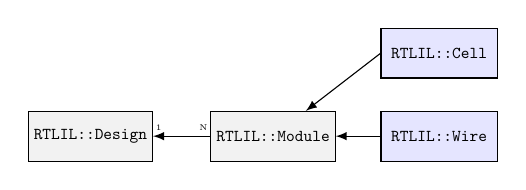
\begin{tikzpicture}[scale=0.6, every node/.style={transform shape}]
	\tikzstyle{entity} = [draw, fill=gray!10, rectangle, minimum height=3em, minimum width=7em, node distance=5em, font={\ttfamily}]
	\node[entity] (design) {RTLIL::Design};
	\node[entity] (module) [right of=design, node distance=11em] {RTLIL::Module} edge [-latex] node[above] {\tiny 1 \hskip3em N} (design);

	\node[entity] (wire) [fill=blue!10, right of=module, node distance=10em] {RTLIL::Wire} (wire.west) edge [-latex] (module);
	\node[entity] (cell) [fill=blue!10, above of=wire] {RTLIL::Cell} (cell.west) edge [-latex] (module);
\end{tikzpicture}
\end{center}

\bigskip
Many command simply choose to only work on this simpler version:
\begin{lstlisting}[xleftmargin=0.5cm, basicstyle=\ttfamily\fontsize{8pt}{10pt}\selectfont]
if (module->processes.size() != 0 || module->memories.size() != 0)
    log_error("This command does not operate on modules with processes "
              "and/or memories! Run 'proc' and 'memory' first.\n");
\end{lstlisting}

\bigskip
So we only discuss this version of RTLIL in this presentation.
\end{frame}



\end{document}
